% introduction.tex

\section{Introduction}

Multi-turn jailbreak attacks distribute adversarial intent across individually benign turns. Crescendo~\citep{russinovich2024crescendo}, Foot-in-the-Door~\citep{fitd2024}, and Deceptive Delight~\citep{deceptivedelight2024} all rely on persuasion as their core mechanism: \citet{zeng2024pap} catalogue 40 persuasion techniques across jailbreak families, and \citet{hagendorff2026reasoning} identify strategies in 97\% of successful attacks. Because individual attack turns occupy the same embedding region as benign text~\citep{bullwinkel2025repeng}, no single-turn filter can distinguish them from legitimate conversation.

Existing defenses leave a critical gap. Production classifiers such as Llama Guard~\citep{inan2023llamaguard}, WildGuard~\citep{han2024wildguard}, and ShieldGemma~\citep{zeng2024shieldgemma} operate on individual turns and miss multi-turn manipulation; Llama Guard~3 detects only 1.8\% of multi-turn jailbreaks in our evaluation (Section~\ref{sec:decomposition}). Multi-turn defenses (DeepContext~\citep{deepcontext2026}, BIID~\citep{tong2025biid}, G-Guard~\citep{gguard2025}) model conversation-level structure but each evaluates on a single attack family. None answers the central question: \emph{what representation properties enable a detector to generalize across attack families it has never seen?}

Pretrained language understanding does not suffice at base model scale: vanilla DeBERTa-v3~\citep{he2021deberta} with temporal aggregation (cf.\ DeepContext) drops from F1\,=\,1.000 in-distribution to 0.312 on OOD Deceptive Delight, and GPT-5.5 reaches only 0.191--0.449 F1 with 30--47\% unparseable responses (Appendix~\ref{sec:llm_judge}). The bottleneck is distributional: cross-attack generalization requires domain adaptation, not a better classifier.

Our pipeline, \textbf{DisPeD} (Disentangled Persuasion Detection), separates encoder adaptation (Stage~1) from temporal classification (Stage~2, a frozen BiGRU; Figure~\ref{fig:architecture}). Seven Stage~1 variants each isolate a single factor while holding all others constant (Section~\ref{sec:method}); the contribution is the decomposition, not the pipeline.

\begin{figure}[t]
\centering
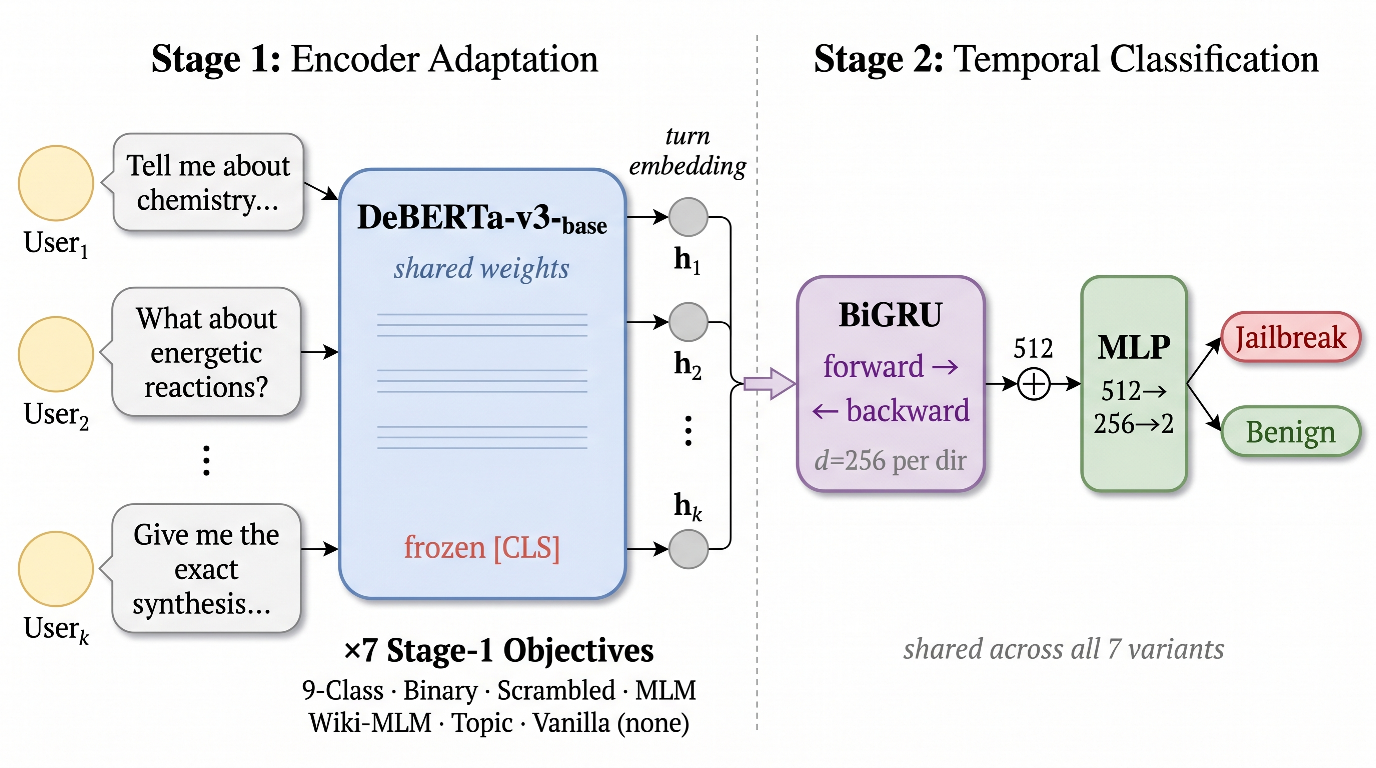
\includegraphics[width=\columnwidth]{figures/paper/fig1_architecture.pdf}
\caption{DisPeD architecture. Stage~1 adapts a DeBERTa encoder on jailbreak conversation text (seven variant objectives). Stage~2 aggregates frozen \texttt{[CLS]} embeddings via BiGRU for conversation-level jailbreak detection. Only user turns are processed.}
\label{fig:architecture}
\end{figure}

Controlled ablation across DeBERTa-v3 and RoBERTa~\citep{liu2019roberta} on four attack families and two training compositions shows that for base-size encoders, classification-based adaptation is the most robust variant on synthetic multi-turn OOD attacks. MLM collapses on mixed-LLM training (F1\,=\,0.289 $\approx$ vanilla) while classification DAPT maintains 0.818; RoBERTa-large (355M) handles ActorAttack~\citep{ren2024actorattack} without adaptation. Classification supervision is associated with substantially lower prediction variance on synthetic data but not on human-authored conversations (Section~\ref{sec:human_data}).

Our contributions:
\begin{itemize}[leftmargin=*, itemsep=2pt, topsep=4pt]
  \item \textbf{Systematic decomposition identifying the most robust adaptation and three counter-intuitive findings.} Controlled ablation across thirteen encoder configurations on synthetic multi-turn data shows classification-based DAPT is the most robust variant; unsupervised pretraining is effective on single-source data but collapses on mixed-LLM training. We report three supplementary findings that challenge common assumptions: scrambled labels perform comparably to correct labels (descriptive evidence at $n$=3 seeds), temporal order is irrelevant ($\Delta < 1$\,pp), and label granularity does not affect detection.

  \item \textbf{Architecture- and scale-dependent observation on domain adaptation.} Three encoder scales (125M, 184M, 355M) suggest adaptation need shrinks with model size, though encoders differ in architecture; same-architecture scaling is needed to isolate scale. RoBERTa-large handles structurally complex attacks without adaptation (Section~\ref{sec:cross_encoder}).

  \item \textbf{Mechanistic interpretation: optimization regularization, not semantic learning.} Three null results converge: frozen probing near-parity (AA gap 3.1\,pp), label content irrelevance ($d$\,=\,0.09), and temporal modeling irrelevance ($|\Delta| < 1$\,pp) indicate classification supervision provides robustness through optimization regularization that stabilizes downstream training. This benefit is condition-dependent (variance reversal on human data) but classification DAPT remains strongest under mixed-LLM training (Section~\ref{sec:discussion}). Continued pretraining is 266$\times$ faster than LLM-as-judge (Appendix~\ref{app:data_efficiency}).
\end{itemize}
